\documentclass{article}
\usepackage[utf8]{inputenc}
\usepackage{graphicx} % Required for inserting images
\usepackage[a4paper, margin=1in]{geometry}
\usepackage[czech]{babel}
\usepackage{setspace}
\usepackage{adjustbox}

\begin{document}

% ÚVODNÍ STRÁNKA
\begin{titlepage}
    \centering
    \Large\textbf{Univerzita Karlova}
    
    \Large{Přírodovědecká fakulta}
    
    \vspace*{2.5cm}
    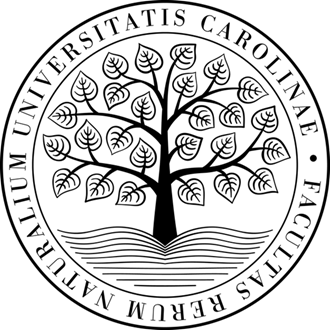
\includegraphics[width=0.55\linewidth]{images/prf.png}
    \vspace*{4cm}
    
    \Large\textbf{ALGORITMY POČÍTAČOVÉ KARTOGRAFIE}
    
    \Large{Geometrické vyhledávání bodu}
    
    \vspace*{3cm}
    \large Martina Pavlová, Martin Šíma, Ludmila Vítková

    1 N-GKDPZ
    
    Praha 2024
\end{titlepage}

% ZADÁNÍ
\begin{spacing}{1.5}
\section*{Zadání}
\subsection*{\textbf{Úloha č. 1: Geometrické vyhledávaní bodu}}
\noindent Vstup: Souvislá polygonová mapa $n$ polygonů \{$P_1, ..., P_n$\}, analyzovaný bod $q$.

\noindent Výstup: $P_i, q \in P_i$.

\noindent Nad polygonovou mapou implementujete Ray Crossing Algorithm pro geometrické vyhledávání incidujícího polygonu obsahujícího zadaný bod $q$.

\noindent Nalezený polygon graficky zvýrazněte vhodným způsobem (např. vyplněním, šrafováním, blikáním). Grafické rozhraní vytvořte s využitím frameworku QT.

\noindent Pro generování nekonvexních polygonů můžete navrhnout vlastní algoritmus či použít existující geografická data (např. mapa evropských států).

\noindent Polygony budou načítány z textového souboru ve Vámi zvoleném formátu. Pro datovou reprezentaci jednotlivých polygonů použijte špagetový model.

\vspace{1cm}
\subsection*{\textbf{Hodnocení}}
\vspace{0.3cm}
\begin{adjustbox}{width=1\textwidth}
%\begin{center}
\begin{tabular}{|l|c|}
\hline
\textbf{Krok}                                                                                  & \textbf{hodnocení} \\ \hline
Detekce polohy bodu rozšiřující stavy uvnitř, vně polygonu.                                    &  10b              \\ \hline
\textit{Analýza polohy bodu (uvnitř/vně) metodou Winding Number Algorithm}                    & \textit{+10b}    \\ \hline
\textit{Ošetření singulárního případu u Winding Number Algorithm: bod leží na hraně polygonu} & \textit{+5b}    \\ \hline
\textit{Ošetření singulárního případu u Ray Crossing Algorithm: bod leží na hraně polygonu}   & \textit{+5b}    \\ \hline
\textit{Ošetření singulárního případu obou algoritmů: bod je totožný s vrcholem jednoho či více polygonů} & \textit{+2b} \\ \hline
\textit{Zvýraznění všech polygonů pro oba výše uvedené singulární případy}                    & \textit{+3b}    \\ \hline
\textit{Rychlé vyhledávání potenciálních polygonů (bod uvnitř min-max boxu)}                    & \textit{+10b}    \\ \hline
\textit{Řešení pro polygony s dírami}                    & \textit{+10b}    \\ \hline
\textbf{Max celkem:}                                                                                  & \textbf{55b} \\ \hline
\end{tabular}
%\end{center}
\end{adjustbox}

\vspace{1cm}
\noindent Řešeny byly všechny bonusové úlohy.
\newpage

\section{Popis a rozbor problému}
Geometrické vyhledávání bodu je často řešeným problémem v oblasti počítačové geometrie a využívá se například v počítačové grafice, geografických informačních systémech a robotice. Tento problém se zabývá lokalizací bodu v geometrickém prostoru, kterým může být například rovina či trojrozměrný prostor a jeho cílem je nalézt určitý bod, který splňuje daná kritéria. Těmi může být například vzdálenost od bodu/polygonu či umístění vůči vymezené oblasti (polygonům). Tento problém může být řešen různými algoritmy, přičemž mezi hojně používané patří Ray Crossing Algorithm a Winding Number Algorithm. Výběr vhodného algoritmu může být ovlivněn velikostí datového souboru či rychlostí vyhledávání. 

\subsection{Ray Crossing Algorithm}
Ray Crossing algoritmus se používá pro zjištění, zda se bod nachází vně, uvnitř či na hraně polygonu. Daným bodem $q$  je vedena polopřímka $r$, která je takzvaným paprskem (ray). Následně se vypočítá kolikrát zvolená polopřímka projde polygonem, přičemž nezáleží na tom, jak byla polopřímka zvolena, avšak často bývá zvolena tak, že má stejnou y-ovou souřadnici jako bod $q$. Pokud je počet průsečíků polopřímky $r$ s polygonem lichý, nachází se bod zvnitř daného polygonu. Naopak pokud je počet průsečíků sudý či roven nule, nachází se bod vně daného polygonu.

\begin{figure}[h]
    \centering
    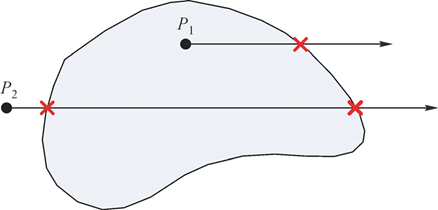
\includegraphics[width=0.7\linewidth]{images/ray.png}
    \caption{Ray Crossing algoritmus (Wang a Benson 2016)}
    \label{fig:enter-label}
\end{figure}

\subsubsection{Problematické situace}
Problém u tohoto algoritmu může nastat v případě, že bod $q$ leží na hraně polygonu. Bod leží na hraně pouze pokud:
$$\|AB\| = \|AP\| + \|PB\|$$
Řešením může být vytvoření vektorů z horizontálních a vertikálních složek rozdílů souřadnic mezi bodem $q$ a přilehlými vrcholy polygonu. Dále se tyto dva vektory sečtou a odečte se od nich délka vektoru reprezentující délku hrany polygonu mezi příslušnými vektory. Tento výsledek se dále porovná s epsilon, což je rozdíl mezi jedničkou a dalším nejmenším číslem větším než 1 (NumPy 2022). Pokud je číslo menší než nejmenší možné číslo, leží bod na hraně polygonu.

Druhá problematická situace nastává, pokud je bod $q$ totožný s vrcholem jednoho či více polygonů. Pro usnadnění výpočtů vytvořen nový souřadnicový systém, který má počátek ve vyhledávaném bodě (paprsek má rovnici $y = 0$ a vyhledáváme pouze průsečíky s $x>0$). Pokud je tedy analyzovaný bod zároveň také lomovým bodem polygonu, má v novém souřadnicovém systému souřadnice [0,0].

\subsubsection{Implementace Ray Crossing algoritmu – pseudokód:}
\noindent Inicializuj proměnnou $k$ pro počítání počtu průsečíků

\noindent Do proměnné $n$ ulož počet bodů v polygon \textit{pol}

\noindent Projdi všechny segmenty polygonů

\indent Vypočítej horizontální složku rozdílu souřadnic mezi bodem a aktuálním vrcholem polygonu

\indent Vypočítej horizontální složku rozdílu souřadnic mezi bodem a následujícím vrcholem polygonu

\indent Vypočítej vertikální složku rozdílu souřadnic mezi bodem a aktuálním vrcholem polygonu

\indent Vypočítej vertikální složku rozdílu souřadnic mezi bodem a následujícím vrcholem polygonu

\indent Pokud bod leží na vrcholu polygonu

\indent\indent Vrať 1

\indent Vytvoř vektory z rozdílů souřadnic

\indent Pokud bod leží na hraně polygonu

\indent\indent Vrať 1

\indent Zkontroluj, zda je úsečka vhodná pro testování průsečíku s paprskem

\indent\indent Vypočti souřadnice průsečíku

\indent\indent Pokud průsečík leží vpravo od bodu

\indent\indent\indent Inkrementuj $k$

\noindent Vrať $k$\%2


\subsection{Winding Number Algorithm}
Winding Number algoritmus se používá k určení kolikrát se daný bod ovine kolem určeného bodu či úsečky v rovině. Je užitečný v případě, kdy chceme zjistit, zda je bod uvnitř nebo vně daného polygonu nebo k detekci průchodu křivky bodem. Funguje na principu, kdy pozorovatel stojí v daném bodě $q$. Pokud bod $q$ leží uvnitř polygonu a chceme z něj vidět celý objekt, musíme se otočit o 360°. Pokud bod $q$ leží vně polygonu bude úhel, o který by se pozorovatel musel otočit menší než 360°. Tento algoritmus pracuje s listem vrcholů polygonu a bodem $q$. Pro každou trojici bodů $q$, $p$ a $p+1$, kdy $p$ je vrchol polygonu a $p+1$ je vrchol následující po $p$ se určí poloha bodu vzhledem k úsečce $p$, $p+1$. Dále se následujícím vzorcem vypočítá úhel $\omega$:

$$\omega = arccos\frac{u*v}{\|u\|*\|v\|}$$

\vspace*{0.3cm}
Pokud se bod nachází v levé polorovině vzhledem k analyzované hraně, tak je úhel přičten k celkové sumě úhlů. Pokud je v pravé, úhel se odečte.
Po zpracování všech hran se od celkové sumy úhlů odečte 2$\pi$. Pokud je výsledkem 0, bod leží uvnitř polygonu.

\begin{figure}[h]
    \centering
    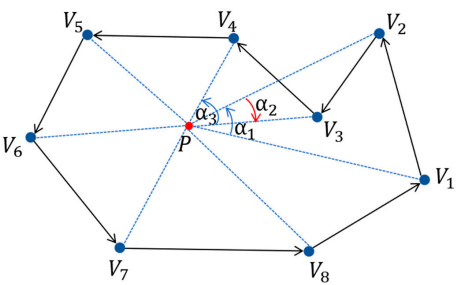
\includegraphics[width=0.7\linewidth]{images/wind.png}
    \caption{Winding Number algoritmus (Liu a kol. 2023)}
    \label{fig:enter-label}
\end{figure}

\subsubsection{Problematické situace}
Stejně jako u Ray Crossing algoritmu i u Winding Number algoritmu mohou nastat problematické situace, kterými jsou situace kdy bod leží na hraně polygonu nebo v jeho vrcholu. Pokud má zadaný bod $q$ stejné souřadnice jako počáteční či koncový bod segmentu polygonu, je automaticky vrácena hodnota 1, která značí, že se bod nachází uvnitř polygonu. Pokud se bod $q$ nenachází ani na počátečním ani na koncovém bodě úsečky, dochází následně ke kontrole, zda se bod $q$ nachází na hraně polygonu. Tato kontrola je realizována porovnáním úhlu mezi dvěma úsečkami, přičemž pokud je tento úhel přibližně $\pi$, leží bod na hraně polygonu a funkce vrátí hodnotu 1.

\subsubsection{Implementace Winding Number algoritmu – pseudokód:}
\noindent Do proměnné \textit{parts} ulož vytvořené segmenty polygonu

\noindent Inicializuj proměnnou $eps$ na hodnotu 1.0e-5

\noindent Inicializuj proměnnou $wn$ na hodnotu 0

\noindent Pro všechny segmenty v $parts$

\indent Inicializuj proměnnou $omega$ na hodnotu

\indent Do proměnné $n$ ulož počet délku aktuální cesty (segmentu)

\indent Projdi všechny segmenty cesty

\indent \indent Do proměnné $startPoint$ přiřaď počáteční bod aktuální hrany

\indent\indent Do proměnné $endPoint$ přiřaď koncový bod aktuální hrany

\indent\indent Pokud je bod $q$ roven počátečnímu či koncovému bodu hrany

\indent\indent\indent Vrať 1

\indent\indent V proměnné $det$ vypočítej determinant pro použití k analýze polohy bodu a hrany

\indent\indent V proměnné $angle$ vypočítej úhel mezi bodem $q$ a segmentem polygonu

\indent\indent\indent Pokud je $det$ menší než $-eps$ 

\indent\indent\indent\indent Přičti $angle$ k $omega$

\indent\indent\indent Jinak pokud je $det$ větší než $eps$

\indent\indent\indent\indent Odečti $angle$ od $omega$

\indent\indent\indent Jinak pokud je $angle$ téměř roven $\pi$

\indent\indent\indent\indent Vrať 1	

\indent Pokud je suma úhlů cca $2\pi$

\indent\indent Zvyš proměnnou $wn$ o 1

\noindent Pokud je bod uvnitř právě jednoho segmentu

\indent Vrať 1

\noindent Vrať 0


\subsection{Min-max box}
Min-max box neboli ohraničující box je jednoduchý geometrický útvar, který obepíná objekt (či skupinu objektů). Tento box je definován celkem čtyřmi body, které mají extrémní hodnoty souřadnic. Jedná se tedy o bod, který má minimální x-ovou a y-ovou souřadnici, bod s maximální x-ovou a minimální y-ovou souřadnicí, bod s maximální x-ovou a y-ovou souřadnicí a bod s minimální x-ovou a maximální y-ovou souřadnicí. Tyto body tedy definují čtyřúhelník, ve kterém se nachází vybraný objekt. 

Tento box se často využívá v počítačové grafice k rychlému zjištění hraničních podmínek objektů. Je rychle vypočitatelný a poskytuje hrubý odhad možných kolizí nebo průsečíků. Například v situaci, kdy hledáme, zda se bod nachází uvnitř nebo vně polygonu, můžeme pomocí min-max boxu eliminovat všechny polygony, které tento box neobsahuje. Tímto krokem lze zrychlit celý algoritmus.

\subsection{Polygony s dírami}
Z důvodu práce s polygony, které mají díry byl pro uložení lomových bodů použit objekt \textit{QPainterPath}. Tento objekt umožňuje uložení více cest do jednoho polygonu. Výhodou je, že lze tyto cesty od sebe odečítat a tím vytvořit díru v polygonu.

Při volbě tlačítka \textit{Make Hole} je po každém kliknutí do mapy vytvořen \textit{QPainerpath} (z dosud naklikaných bodů), který je poté odečten od všech polygonů (byla vytvořena díra). Při samotném vyhledávání polygonů, které obsahují zadaný bod, se \textit{QPainterPath} rozdělí zpět na jednotlivé cesty (okraj polygonu, díra) pomocí metody \textit{toSubpathPolygons}. Tyto cesty byly poté procházeny stejným způsobem jako při použití \textit{QPolygonF}. Tyto části jsou posléze zpracovány jednotlivě.

V případě Ray Crossing nemá vliv počet „cest“ v polygonu. U Winding Number je však nutné detekovat polohu bodu vůči všem „cestám“. V grafickém rozhraní není možné vytvořit polygon uvnitř polygonu s dírou. Tudíž bod leží uvnitř polygonu (i polygonu s dírou) pokud je uvnitř právě jedné z „cest“. Pokud je bod uvnitř libovolné cesty, je inkrementována pomocná proměnná. Pokud má tato proměnná, po zpracování všech cest, hodnotu 1 (bod je uvnitř právě jedné cesty), bod se nachází uvnitř polygonu.

\section{Struktura programu}
Tento program se skládá ze 7 souborů kterými jsou \textit{Algorithms.py}, \textit{Load.py}, \textit{MainForm.py}, \textit{Polygon.py}, \textit{draw.py} a složky \textit{Data} a \textit{images}. 

Ve složce Data se nacházejí vstupní data pojmenována \textit{Polygons.json}. Tato data tvoří souvislá polygonová mapa ve formátu JSON, která má celkem 76 polygonů, jelikož reprezentuje okresy České republiky. Ve vstupních datech jsou dva hlavní klíče \textit{COUNTER}, který obsahuje počet polygonů a \textit{POLYGONS}, který obsahuje seznam polygonů. Každý polygon je reprezentován jako objekt obsahující klíče \textit{ID}, který označuje identifikátor polygonu a \textit{POINTS}. Druhý zmíněný klíč obsahuje seznam bodů tvořících hranice polygonu, přičemž každý bod je reprezentován jako dvojice souřadnic [x, y], které jsou zadané jako desetinná čísla s devíti desetinnými místy. Souřadnice jsou zadané v Křovákově zobrazení. Ve složce je ještě druhý soubor pojmenován \textit{Polygons\_holes}, který obsahuje pouze dva polygony s jednou dírou. Formát vstupních dat je stejný jako u souboru \textit{Polygons}.

Ve složce \textit{images} se nachází další složka \textit{icons}, ve které jsou uloženy ikony pro tvoření aplikace. Těmito ikonami jsou soubory \textit{about.png}, \textit{clear.png}, \textit{clear\_all.png}, \textit{exit.png}, \textit{open\_file.png}, \textit{pointpol.png}, \textit{ray.png} a \textit{Winding.png}. 

V \textit{Algorithms.py} je definována třída \textit{Algorithms}, která obsahuje několik metod. Metoda \textit{preProcessPolygons} zajišťuje rychlé vyhledávání potenciálních polygonů. Tato metoda přijímá bod $q$ a seznam polygonů \textit{polygons} a vrací seznam indexů polygonů, které obsahují bod $q$ ve svém min-max boxu. Další metodou je \textit{rayCrossingAlgorithm}, která implementuje Ray Crossing algoritmus pro učení toho, zda bod $q$ leží uvnitř nebo vně polygonu. Tato metoda přijímá bod $q$ a polygon \textit{pol} a vrací 1, pokud se bod nachází uvnitř polygonu. Pokud se bod nenachází uvnitř polygonu, vrací hodnotu 0. Metoda \textit{windingNumber} má stejný úkol jako předchozí metoda, a to určit, zda se daný bod nachází uvnitř či vně polygonu. Stejně jako v předchozím případě i tato metoda přijímá bod $q$ a polygon $pol$ a vrací 1 či 0 v závislosti na poloze bodu. Čtvrtou metodou je \textit{angleTwoLine}, která jako vstupní parametry přijímá tři body, kterými jsou analyzovaný bod $q$, \textit{startPoint} a \textit{endPoint} (body určující úsečku). Nejprve dojde k vypočítání vektorů, poté k vypočítání jejich délek, dále ke skalárnímu součinu vektorů, a nakonec k výpočtu úhlu. Poslední metodou je \textit{pointEdgePosition}, která přijímá stejné vstupní parametry jako metoda předchozí a slouží k určení polohy bodu vzhledem k úsečce.

V \textit{Load.py} dochází k načtení vstupních dat pomocí funkce \textit{load\_polygons}. Nejprve je soubor otevřen pomocí \textit{json.load()} a uložen do proměnné \textit{file}. Poté jsou do proměnné \textit{polygons} uloženy všechny polygony ze vstupního souboru. Pro každý polygon se vypočítá jeho minimální a maximální x-ová a y-ová souřadnice. Dále dochází ke zpracování polygonů tak, aby se vešly do určeného zobrazovacího okna. Pomocí funkce \textit{transformPolygons} dojde k transformování souřadnic jednotlivých polygonů, které se následně převedou na objekty typu \textit{QPainterPath}. Posledním krokem je vytvoření děr v polygonech pomocí jejich odečtení. Funkce \textit{transformPoylgons} trasnformuje souřadnice polygonů do nových souřadnic, které jsou kompatibilní se souřadnicemi plátna, na které se mají polygony vykreslit. 

V \textit{MainForm.py} je definována třída \textit{Ui\_MainWindow}, ve které je následně definováno několik metod. Metody \textit{setupUI} a \textit{retranslateUI} byly vygenerovány v prostředí Qt. Nově implementovanými byly metody \textit{openClick}, \textit{pointPolygonClick}, \textit{rayCrossing}, \textit{windingNumber} a \textit{clear}. Zavolání metody \textit{openClick} proběhne při kliknutí na možnost \textit{Open} v menu. Dochází k otevření dialogového okna pro výběr souboru typu JSON a po výběru souboru dojde pomocí funkce \textit{load\_polygons} k načtení polygonů, které jsou následně vykresleny. Po kliknutí na možnost \textit{Make Hle} v menu je zavolána metoda \textit{makeHo}, která umožňuje vytvořit díru v načtených polygonech, klikáním lze přidat lomové body díry. Metoda \textit{rayCrossing} je zavoláno po kliknutí na možnost \textit{Ray Crossing Algorithm} v menu a získává souřadnici bodu $q$ a seznam polygonů. V případě, že jsou souřadnice bodu kladné a současně jsou načtené polygony, provede analýzu pozice bodu vůči polygonům pomocí Ray Crossing algoritmu. Pokud se zadaný bod nachází v některém z polygonů, je tento polygon zvýrazněn červenou barvou. Pokud je tato metoda zavolána dříve, než byl vybrán bod $q$ nestane se nic. Po kliknutí na \textit{Winding Number Algorithm} v menu dojde k zavolání metody \textit{windingNumber}. Stejně jako předchozí metoda provede analýzu pozice bodu vůči polygonům, avšak v tomto případě za použití Winding Number algoritmu. Opět platí, že pokud se bod nachází v polygonu, dojde ke zvýraznění daného polygonu a že pokud nebyl vybrán žádný bod, nestane se nic. Předposlední metodou je \textit{clear}, která je zavolána kliknutím na možnost \textit{Clear} v menu. Tato metoda vyčistí plátno tak, že vymaže načtené polygony a souřadnice bodu $q$ nastaví na výchozí hodnotu. Následně ještě dojde k překreslení plátna, aby se změny projevily. Poslední metoda \textit{makeHole} přepíná režim kreslení z bodu na díru.

\textit{Polygon.py} obsahuje třídu \textit{Polygon}, ve které jsou obsažené metody pro manipulaci s polygonem. Počet vrcholů polygonu vrací přetížená build-in funkce \textit{len()} a přístup k vrcholům polygonu pomocí indexu umožňují přetížené hranaté závorky \textit{[]}. Metoda \textit{addVertex} přidá nový vrchol k polygonu, metoda \textit{isInMMB} určuje, zda je daný bod uvnitř min-max boxu polygonu a metoda \textit{updateMMB} aktualizuje min-max box polygonu na základě nového vrcholu. Poslední metodou je \textit{convertPolToPath}, která konvertuje objekt \textit{QPolygonF} na objekt \textit{QPainterPath}. 

V \textit{draw.py} se nachází třída \textit{Draw}, ve které je definovaných šest různých metod. Metoda \textit{switchDrawing} slouží k přepínání mezi režimem kreslení bodů a polygonů na plátně. Metoda \textit{getPols} slouží k získání seznamu polygonů, které jsou vykresleny na plátně a současně vrací aktuální seznam polygonů. Pomocí \textit{getQ} dochází k získání souřadnic aktuální pozice bodu $q$. K vyčištění plátna slouží metoda \textit{clearData}, která nastavuje seznam polygonů na prázdný, seznam indexů průsečíků na prázdný a souřadnice bodu $q$ na [-100, -100], což způsobí, že se bod $q$ nevykreslí na plátno. Metoda \textit{mousePressEvent} je zavolána při stisknutí tlačítka myši na plátně a s její pomocí lze získat souřadnice daného bodu $q$. Dále slouží k přidání díry do polygonu a vložení bodu. Poslední metodou je \textit{paintEvent}, která je volána při každém vykreslení plátna. Dojde k vykreslení polygonů a bodu $q$ na plátno, kde polygonu mají červený okraj a zelenou výplň a bod $q$ je žlutý. 

\section{Výsledky}
V rámci této úlohy došlo k vytvoření uživatelského rozhraní s využitím frameworku QT, ve kterém je demonstrována funkčnost algoritmů Ray Crossing a Winding Number na polygonové mapě. Toto grafické rozhraní aplikace vytvořené v prostředí Qt Designer lze vidět na obrázku 3 a dále bylo upravováno v prostředí programovacího jazyka Python. Po spuštění aplikace může uživatel otevřít soubor obsahující polygony a následně v těle aplikace pomocí kliknutí levým tlačítkem myši přidat vlastní bod $q$, aby mohlo dojít k analýze jeho polohy vůči vstupním datům.

\begin{figure}[h]
    \centering
    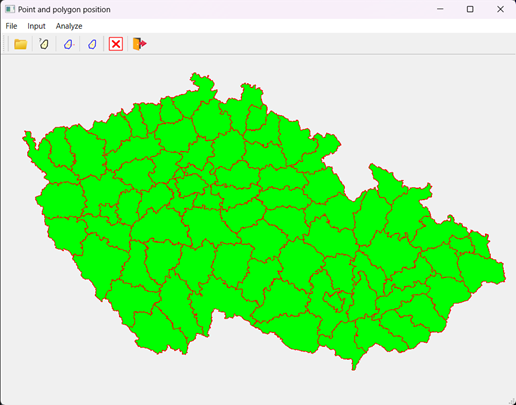
\includegraphics[width=0.62\linewidth]{images/app01.png}
    \caption{Grafické rozhraní aplikace po načtení souboru s polygony}
    \label{fig:enter-labe}
\end{figure}

V rámci tohoto rozhraní lze zvolit, kterou metodou budou objekty analyzovány. Po zvolení metody \textit{Ray Crossing Algorithm} či \textit{Winding Number Algorithm} proběhne analýza dat a dojde ke zvýraznění polygonu, ve kterém se zadaný bod $q$ nachází. Polygony vstupních dat mají barvu zelenou, zatímco polygon, ve kterém se daný bod $q$ nachází se zvýrazní barvou červenou. Výsledek analýzy lze vidět na obrázku 4.

\begin{figure}[h]
    \centering
    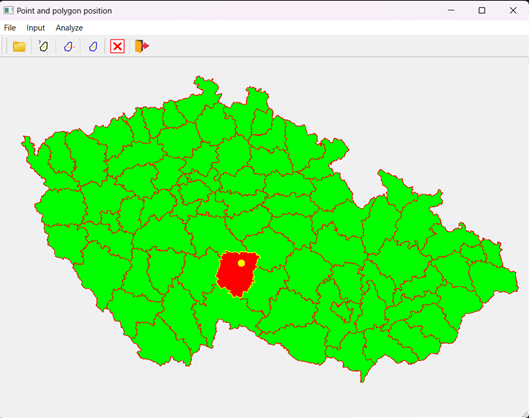
\includegraphics[width=0.62\linewidth]{images/app02.png}
    \caption{Výsledek analýzy – zvýraznění polygonu obsahující bod q}
    \label{fig:enter-label}
\end{figure}
V případě, že se bod nenachází v žádném ze vstupních polygonů, dojde k otevření dialogového okna, které lze vidět na obrázku 5. Toto okno informuje uživatele, že zadaný bod $q$ neprotíná žádný ze vstupních polygonů. 

\begin{figure}[h]
    \centering
    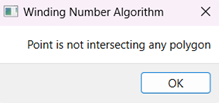
\includegraphics[width=0.3\linewidth]{images/app03.png}
    \caption{Dialogové okno otevřené v případě, kdy se bod nenachází v žádném z polygonů}
    \label{fig:enter-label}
\end{figure}

Pokud v možnosti \textit{Input} zvolíme \textit{Make hole}, můžeme ve vstupním souboru polygonů vytvořit libovolné díry. Výsledek může vypadat například jako na obrázku 6.

\begin{figure}[h]
    \centering
    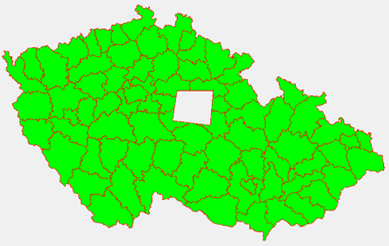
\includegraphics[width=0.6\linewidth]{images/app04.png}
    \caption{Výsledek polygonů s dírou}
    \label{fig:enter-label}
\end{figure}

\section{Závěr}
V rámci této úlohy došlo k představení a implementování algoritmů Ray Crossing a Winding Number, které mohou sloužit pro analýzu pozice bodu vůči polygonům. Jako vstupní data byla použita souvislá polygonová mapa ve formátu JSON a analyzovaný bod $q$. Celý postup analýzy objektů lze provést ve vzniklém grafickém rozhraní s využitím frameworku QT, kde může uživatel vybrat kterou metodou chce vstupní data analyzovat. Výstupem je zvýraznění polygonu (či polygonů), ve kterém se daný bod nachází. Program zvládá také určit, zda se bod nachází na hraně či ve vrcholu polygonu. Pokud se bod nachází ve vrcholu nebo na hraně polygonu, zvládá program správně určit jeho příslušnost k danému polygonu.


\newpage
\section*{Seznam literatury: }
LIU, L., SUN, Y., JI, M., WANG, H., LIU, J. (2023): Efficient Construction of Voxel Models for Ore Bodies Using an Improved Winding Number Algorithm and CUDA Parallel Computing. International Journal of Geo-Information, 12, 473.

\vspace*{0.5cm}
\noindent NumPy (2022): Numpy finfo, NumPy, https://numpy.org/doc/stable/reference/generated/numpy.finfo.html
(23. 3. 2024).

\vspace*{0.5cm}
\noindent WANG, Y., BENSON, D. J. (2016): Geometrically constrained isogeometric parametrized level-set topology optimization via trimmed elements. Frontiers of Mechanical Engineering, 11, 1-16. 

\end{spacing}
\end{document}
